\section{Entwurfsdaten}

In diesem Kapitel werden die Daten, die für die Software benötigt werden bzw. von ihr gespeichert werden, aufgeführt.

\subsection{Ressourcen}
Zur Darstellung der Webseite werden HTML-Dateien für den Aufbau der Seiten und CSS-Dateien für den Style der Seiten benötigt.
Diese werden im resources-Ordner mit folgender Struktur gespeichert.

\begin{figure}[htbp]
\centering
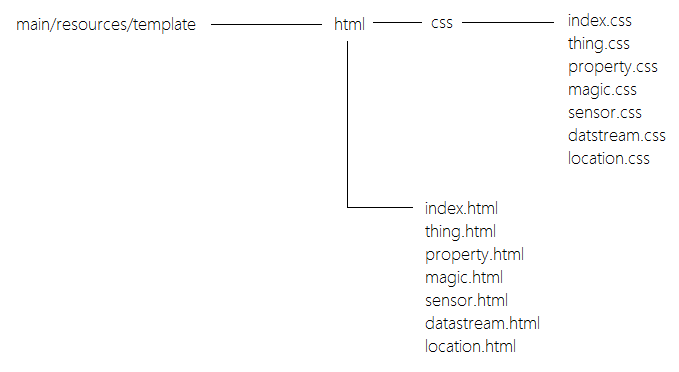
\includegraphics[scale=0.8]{images/resources.png}
\caption{Ordnerstruktur der Ressourcen}
\end{figure}

\subsection{Dateneinträge}
Für den fehlerlosen Ablauf der Software müssen einige veränderlichen Daten auf dem Server zwischengespeichert werden.
Dazu gehört Folgendes:
\begin{itemize}
\item Kopie der Quelldatei
\item Gespeicherte Konfigurationen
\item Datei mit fehlerhaften Zeilen zur Rückgabe
\end{itemize}